\documentclass[border=3mm]{standalone}

\usepackage{tikz}
\usetikzlibrary{arrows.meta,decorations.markings,calc,intersections,backgrounds}

\begin{document}
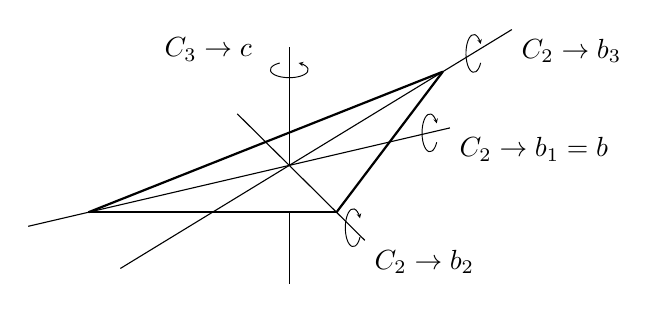
\begin{tikzpicture}[scale=0.75]
\newcommand{\AxisRotator}[1][rotate=0]{% Defining symbol for axes rotations
    \tikz [x=0.25cm,y=0.60cm,line width=.2ex,-stealth,#1] \draw (0,0) arc (-150:150:1 and 1);%
}

\fill[white] (-6.4,-1.6) -- (-2.2,-1.6) -- (-0.4,0.78) -- cycle;

% Drawing triangle and defining mid-points of each side
\draw[thick] (-6.4,-1.6) coordinate (1)  -- (-2.2,-1.6) coordinate (3) coordinate[pos=0.5] (6);
\draw[thick] (-2.2,-1.6) -- (-0.4,0.78) coordinate[pos=0.5](2);
\draw[thick] (-0.4,0.78)coordinate (5) -- (-6.4,-1.6) coordinate[pos=0.5](4);

% For finding center of triangle
\draw[name path=A] ($(1)!-.2!(2)$) -- ($(2)!-.2!(1)$) node[pos=0.95,scale=0.4,xscale=-1]{\AxisRotator} node[below right] {$C_2 \rightarrow b_1 = b$};
\draw[name path=B] ($(3)!-.4!(4)$) node[below right] {$C_2 \rightarrow b_2$} -- ($(4)!-.4!(3)$) node[pos=0.1,scale=0.4,xscale=-1]{\AxisRotator};

\draw ($(5)!-.3!(6)$) node[below right] {$C_2 \rightarrow b_3$} -- ($(6)!-.4!(5)$) node[pos=0.1,scale=0.4,xscale=-1]{\AxisRotator};
\path[name intersections={of=A and B}] (intersection-1) coordinate (c);
\draw (c) --++ (0,2) node[pos=0.8,rotate=-90,scale=0.4] {\AxisRotator} node[pos=0.8,above left,xshift=-10pt]{$C_3 \rightarrow c$};
\begin{scope}[on background layer]
\draw (c) --++ (0,-2);
\end{scope}
\end{tikzpicture}
\end{document}
